\documentclass[pdftex,10pt,xcolor=svgnames]{beamer}

\mode<presentation>
{
  \usetheme{boxes}
  \usecolortheme[named=MidnightBlue]{structure}
  %\setbeamercolor{normal text}{bg=NavajoWhite!20}
  \usefonttheme{serif}
  \setbeamertemplate{navigation symbols}{}
  % Show frame number and author name in footline
  \setbeamertemplate{footline}[frame number]
  \addtobeamertemplate{footline}{\quad\textcolor{gray}{James Lloyd}}{}
  % Set frame titles in small capitals
  \setbeamerfont{frametitle}{shape=\scshape,family=\rmfamily}
  \setbeamercolor{frametitle}{bg=gray!60!white,fg=black}
  % Alerted text: blue (uncomment second line if theme sets alerted text to bold)
  \setbeamercolor{alerted text}{fg=blue}
  %\setbeamerfont*{alerted text}{}
  \setbeamertemplate{bibliography item}[text] %{\hbox{\donotcoloroutermaths$\blacktriangleright$}}
  \setbeamertemplate{bibliography entry title}{}
  \setbeamertemplate{bibliography entry author}{}
  \setbeamertemplate{bibliography entry note}{}
  \setbeamertemplate{bibliography entry location}{}

}
\usepackage[english]{babel}
\usepackage[latin1]{inputenc}
\usepackage{times}
\usepackage[T1]{fontenc}
\usepackage{hyperref}
\usepackage{multimedia}
\usepackage{eepic}
\usepackage{graphicx}
%\usepackage[nohug]{latexinclude/diagrams}
\usepackage{tikz}
\usetikzlibrary{calc}

%% \newcommand{\footlineextra}[1]{
%%     \begin{tikzpicture}[remember picture,overlay]
%%         \node[yshift=1.5ex,anchor=south east] at (current page.south east)
%% {#1};
%%     \end{tikzpicture}
%% }

\newcommand{\footlineextra}[1]{
    \begin{tikzpicture}[remember picture,overlay]
        \node[xshift=-5ex,yshift=-0.5ex,anchor=south east] at (current page.south east)
             {\mbox{\tiny \textcolor{MidnightBlue}{#1}}};
    \end{tikzpicture}
}

\def\sectionframe#1{
  {
    \setbeamertemplate{footline}{\empty}
    \begin{frame}{}
      \begin{center}
        \huge\sc #1
      \end{center}
    \end{frame}
  }
}



\usecolortheme{default}
\xdefinecolor{Black}{rgb}{0,0,0}
\xdefinecolor{White}{rgb}{1,1,1}
\xdefinecolor{DarkBlue}{rgb}{0,0,.7}
\xdefinecolor{DarkRed}{rgb}{.7,0,0}
\xdefinecolor{Red}{rgb}{.85,0,0}
\xdefinecolor{DarkGreen}{rgb}{0,.7,0}
\xdefinecolor{DarkMagenta}{rgb}{.6,0,.6}
\def\Black{\textcolor{Black}}
\def\White{\textcolor{White}}
\def\Blue{\textcolor{DarkBlue}}
\def\Magenta{\textcolor{DarkMagenta}}
\def\Red{\textcolor{Red}}
\def\Green{\textcolor{DarkGreen}}
\definecolor{camlightblue}{rgb}{0.601 , 0.8, 1}

\usepackage{alltt}
\usepackage{psfrag}
\usepackage{pstool}

\def\newarrow{\mbox{\begin{tikzpicture}
             \useasboundingbox{(-3pt,-4.5pt) rectangle (19pt,1pt)};
             \draw[->] (0,-0.07)--(17pt,-0.07);\end{tikzpicture}}}

\title[] % (optional, use only with long paper titles)
{The Aldous--Hoover representation theorem and applications to modeling relational data}

\author % (optional, use only with lots of authors)
{James Lloyd}
% - Use the \inst{?} command only if the authors have different
%   affiliation.

\institute[] % (optional, but mostly needed)
{University of Cambridge}
% - Use the \inst command only if there are several affiliations.
% - Keep it simple, no one is interested in your street address.

\date % (optional)
{January 2013}

\subject{Talks}

\usetikzlibrary{shapes.geometric,arrows,chains,matrix,positioning,scopes}
 \makeatletter
 \tikzset{join/.code=\tikzset{after node path={%
       \ifx\tikzchainprevious\pgfutil@empty\else(\tikzchainprevious)%
       edge[every join]#1(\tikzchaincurrent)\fi}}
 }
 \tikzset{>=stealth',every on chain/.append style={join},
   every join/.style={->}
 }

\tikzstyle{mybox} = [draw=white, rectangle]
\usepackage{ifthen}
\usepackage{booktabs}

% Custom definitions
\def\simiid{\sim_{\mbox{\tiny iid}}}

%%%%%%%%%%%%%%%%%%%%%%%%%%%%%%%%%%%%%%%%%%%%%%%%%%%%%%%%%%
%%%% EDITING HELPER FUNCTIONS  %%%%%%%%%%%%%%%%%%%%%%%%%%%
%%%%%%%%%%%%%%%%%%%%%%%%%%%%%%%%%%%%%%%%%%%%%%%%%%%%%%%%%%

%% NA: needs attention (rough writing whose correctness needs to be verified)
%% TBD: instructions for how to fix a gap ("Describe the propagation by ...")
%% PROBLEM: bug or missing crucial bit 

%% use \fXXX versions of these macros to put additional explanation into a footnote.  
%% The idea is that we don't want to interrupt the flow of the paper or make it 
%% impossible to read because there are a bunch of comments.

%% NA's (and TBDs, those less crucially) should be written so 
%% that they flow with the text.

\definecolor{WowColor}{rgb}{.75,0,.75}
\definecolor{SubtleColor}{rgb}{0,0,.50}

% inline
\newcommand{\NA}[1]{\textcolor{SubtleColor}{ {\tiny \bf ($\star$)} #1}}
\newcommand{\LATER}[1]{\textcolor{SubtleColor}{ {\tiny \bf ($\dagger$)} #1}}
\newcommand{\TBD}[1]{\textcolor{SubtleColor}{ {\tiny \bf (!)} #1}}
\newcommand{\PROBLEM}[1]{\textcolor{WowColor}{ {\bf (!!)} {\bf #1}}}

% as margin notes

\newcounter{margincounter}
\newcommand{\displaycounter}{{\arabic{margincounter}}}
\newcommand{\incdisplaycounter}{{\stepcounter{margincounter}\arabic{margincounter}}}

\newcommand{\fTBD}[1]{\textcolor{SubtleColor}{$\,^{(\incdisplaycounter)}$}\marginpar{\tiny\textcolor{SubtleColor}{ {\tiny $(\displaycounter)$} #1}}}

\newcommand{\fPROBLEM}[1]{\textcolor{WowColor}{$\,^{((\incdisplaycounter))}$}\marginpar{\tiny\textcolor{WowColor}{ {\bf $\mathbf{((\displaycounter))}$} {\bf #1}}}}

\newcommand{\fLATER}[1]{\textcolor{SubtleColor}{$\,^{(\incdisplaycounter\dagger)}$}\marginpar{\tiny\textcolor{SubtleColor}{ {\tiny $(\displaycounter\dagger)$} #1}}}


%% For submission, make all render blank.
%\renewcommand{\LATER}[1]{}
%\renewcommand{\fLATER}[1]{}
%\renewcommand{\TBD}[1]{}
%\renewcommand{\fTBD}[1]{}
%\renewcommand{\PROBLEM}[1]{}
%\renewcommand{\fPROBLEM}[1]{}
%\renewcommand{\NA}[1]{#1}  %% Note, NA's pass through!

%%%%
% Paper specific stuff
%%%%

\newtheorem{thm}{Theorem}%[section]
\newtheorem{lem}[thm]{Lemma}
\newtheorem{prop}[thm]{Proposition}
\newtheorem{cor}[thm]{Corollary}

\newtheorem*{theorem*}{Theorem}

\theoremstyle{definition}
\newtheorem*{definition*}{Definition}
%\newtheorem{definition}[thm]{Definition}%[section]
\newtheorem{conj}{Conjecture}[section]
\newtheorem{exmp}{Example}[section]
\newtheorem{rem}[thm]{Remark}

\theoremstyle{remark}
%\newtheorem{rem}{Remark}
%\newtheorem{note}{Note}
%\newtheorem{case}{Case}

\newcommand{\eqd}{\overset{\,_{\!d}}{=}}
\newcommand{\defn}[1]{\emph{#1}}

\newcommand{\Law}{\mathcal{L}}

\def\given{\,|\,}

\def\SGinf{\mathbb{S}_{\infty}}

\newcommand{\NonNegInts}{\mathbb{Z}_+}
\newcommand{\Nats}{\mathbb{N}}
\newcommand{\Rationals}{\mathbb{Q}}
\newcommand{\Reals}{\mathbb{R}}

\newcommand{\as}{\textrm{a.s.}}

\def\[#1\]{\begin{align}#1\end{align}}
\newcommand{\defas}{:=}

\newcommand{\Normal}{\mathcal{N}}
\newcommand{\dist}{\ \sim\ }

\newcommand{\kernel}{\kappa}
\newcommand{\kernelmatrix}{K}
\newcommand{\scalefactor}{s}
\newcommand{\lengthscale}{\ell}
\newcommand{\targets}{T}
\newcommand{\noise}{\sigma_\targets}
\newcommand{\pseudopoints}{\eta}
\newcommand{\inputpoints}{\xi}
\newcommand{\covhyppar}{\psi}
\newcommand{\logistic}{\phi}

\newcommand{\CompOrder}{\mathcal{O}}
\def\graphspace{\mathbf{G}}
\def\Uniform{\mbox{\rm Uniform}}
\def\Bernoulli{\mbox{\rm Bernoulli}}
\def\ie{i.e.,\ }
\def\eg{e.g.,\ }
\def\iid{i.i.d.\ }
\def\simiid{\sim_{\mbox{\tiny iid}}}
\def\simind{\sim_{\mbox{\tiny ind}}}
\def\eqdist{\stackrel{\mbox{\tiny d}}{=}}
\def\ahfunction{\theta}       
\def\AHfunction{\Theta}           % A-H random function
\def\AHvar{U}                     % A-H uniform variables
\def\AHvaralt{V}                  % A-H uniform variables - for bipartite data
\def\larray{W}                    % latent array sampled with A-H
%\def\latentspace{\mathbf{W}}      % range of entries
\def\latentspace{\mathcal{W}}      % range of entries
\def\darray{X}                    % data array
%\def\dataspace{\mathbf{X}}        % sample space
\def\dataspace{\mathcal{X}}        % sample space
\def\cfspace{\mathbf{C}}          % space of continuous functions
%\def\GP{\mbox{\mathcal{GP}}}
\def\GP{\mathcal{GP}}
\def\likelihood{P}
\def\CovData{C}
\def\CovDataAlt{D}

\begin{document}

\small
%% { 
%%   \setbeamertemplate{footline}{\empty}
%%   \begin{frame}
%%     \titlepage
%%   \end{frame}
%% }
\renewcommand{\inserttotalframenumber}{11}

%\theoremstyle{plain}

\def\ie{i.e.\ }
\def\eg{e.g.\ }
\def\indicator{\mathbb{I}}
\def\mean#1{\mathbb{E}[#1]}
\def\bigmean#1{\mathbb{E}\bigl[#1\bigr]}
\def\Bigmean#1{\mathbb{E}\Bigl[#1\Bigr]}
\def\cyl{\mathcal{Z}}
\def\eqae{=_{\mbox{\tiny a.e.}}}
\def\wrt{w.r.t.\ }
\def\ae{a.e.\ }
\def\equas{=_{\mbox{\tiny a.s.}}}
\def\equae{=_{\mbox{\tiny a.e.}}}
\def\iid{i.i.d.\ }
\def\Iid{I.i.d.\ }
%\def\inclusion{\jmath}
\def\inclusion{\mathcal{J}}
\def\inclusionX{\inclusion_{\xspace}}
\def\wstar{weak$^{\ast}$ }
% Symmetric difference
\def\symmdiff{\!\vartriangle\!}


% Indices

\def\indI{\mbox{\tiny I}}
\def\indJ{\mbox{\tiny J}}
\def\indK{\mbox{\tiny K}}
\def\indJI{\mbox{\tiny J$\setminus$I}}
\def\indE{\mbox{\tiny E}}
\def\indF{\mbox{\tiny F}}
\def\indD{\mbox{\tiny D}}
\def\indi{\mbox{\tiny{\{i\}}}}
\def\ind#1{\mbox{\tiny #1}}
\def\power{\mathcal{F}}
\def\powerD{\power(D)}
\def\powerE{\power(E)}
\def\powerL{\power(L)}
\def\parts{\mathcal{H}}
\def\partsQ{\parts(\mathcal{Q})}
\def\partsn{\parts[n]}
\def\partsN{\parts_{\infty}(\mathbb{N})}

% Spaces

\def\abstspace{\Omega}
\def\xspace{\mathcal{X}}
\def\yspace{\mathcal{Y}}
\def\tspace{\mathcal{T}}
\def\xspaceI{\xspace_{\indI}}
\def\xspaceJ{\xspace_{\indJ}}
\def\xspaceD{\xspace_{\indD}}
\def\xspaceE{\xspace_{\indE}}
\def\tspaceI{\tspace_{\indI}}
\def\tspaceJ{\tspace_{\indJ}}
\def\tspaceD{\tspace_{\indD}}
\def\tspaceE{\tspace_{\indE}}
\def\txspace{\tilde{\xspace}}
\def\yspaceI{\yspace_{\indI}}
\def\yspaceJ{\yspace_{\indJ}}
\def\yspaceD{\yspace_{\indD}}
\def\yspaceE{\yspace_{\indE}}
\def\txspace{\tilde{\xspace}}
\def\ttspace{\tilde{\tspace}}
\def\xI{x_{\indI}}
\def\xJ{x_{\indJ}}
\def\xD{x_{\indD}}
\def\xE{x_{\indE}}
\def\tImage{\Gamma}
\def\simp{\triangle}
\def\simpI{\simp_{\indI}}
\def\simpJ{\simp_{\indJ}}

\def\AI{A_{\indI}}
\def\AJ{A_{\indJ}}
\def\AD{A_{\indD}}
\def\AE{A_{\indE}}


%Space of Prob Measures
\def\pMeas{M}
%Space of Contents
\def\fMeas{N}
%Space of cont fcts
\def\cfspace{C}
%Hilbert space
\def\hilbert{\mathcal{L}^2}


\def\borelV{\borel_{V}}

% Set systems

\def\borel{\mathcal{B}}
\def\top{\mbox{Top}}

\def\borelI{\borel_{\indI}}
\def\borelJ{\borel_{\indJ}}
\def\borelD{\borel_{\indD}}
\def\borelE{\borel_{\indE}}
\def\tborel{\tilde{\borel}}
\def\abstfield{\mathcal{A}}
\def\field{\mathcal{C}}
\def\fieldI{\field_{\indI}}
\def\fieldJ{\field_{\indJ}}
\def\fieldK{\field_{\indK}}
\def\fieldD{\field_{\indD}}
\def\fieldE{\field_{\indE}}
\def\tfield{\tilde{\mathcal{C}}}
\def\Sfield{\mathcal{S}}
\def\SfieldI{\mathcal{S}_{\indI}}
\def\SfieldJ{\mathcal{S}_{\indJ}}
\def\SfieldD{\mathcal{S}_{\indD}}
\def\tSfield{\tilde{\mathcal{S}}}
\def\borelx{\borel_x}
\def\tborelx{\tborel_x}
\def\borelgamma{\tborel_{\tImage}}
%\def\borelth{\borel_{\theta}}
\def\borely{\borel_{y}}
%\def\borelT{\borel_t}
\def\borelT{\borel_{\tspace}}
\def\borelS{\borel_s}
\def\topI{\top_{\indI}}
\def\topJ{\top_{\indJ}}
\def\topD{\top_{\indD}}
\def\topE{\top_{\indE}}
\def\topV{\top_V}
\def\topws{\top_{\text{ws}}}
\def\topcc{\top_{\text{c}}}
\def\borelXI{\borel(\xspaceI)}
\def\borelXD{\borel(\xspaceD)}
\def\tborelX{\borel(\txspace)}
\def\borelTI{\borel(\tspaceI)}
\def\borelTD{\borel(\tspaceD)}
\def\tborelT{\borel(\ttspace)}


% Maps

\def\XI{X_{\indI}}
\def\Xi{X_{\ind{i}}}
\def\Xj{X_{\ind{j}}}
\def\ThetaI{\Theta_{\indI}}
\def\XJ{X_{\indJ}}
\def\ThetaJ{\Theta_{\indJ}}
\def\XD{X_{\indD}}
\def\ThetaD{\Theta_{\indD}}
\def\XE{X_{\indE}}
\def\ThetaE{\Theta_{\indE}}
\def\tX{\tilde{X}}
\def\tTheta{\tilde{\Theta}}

\def\SI{S_{\indI}}
\def\TI{T_{\indI}}

\def\rest{\phi}
\def\restD{\rest_{\indD}}
\def\restI{\rest_{\indI}}
\def\restJ{\rest_{\indJ}}
\def\restDI{\rest^{\indD}_{\indI}}
\def\inclusionD{\inclusion_{\indD}}
\def\inclusionE{\inclusion_{\indE}}
\def\projector{\mbox{pr}}
\def\projectorD{\projector_{\indD}}
\def\projectorI{\projector_{\indI}}
\def\projectorJI{\pi_{\indJ\indI}}
\def\indicator{\mathbb{I}}

% Projective systems

\def\po{\preceq}
\def\famD#1{{\lbrace #1 \rbrace}_{\indD}}
\def\famE#1{{\lbrace #1 \rbrace}_{\ind{I$\in$}\indE}}
\def\fJI{f_{\indJ\indI}}
\def\fKI{f_{\indK\indI}}
\def\fKJ{f_{\indK\indJ}}
\def\fII{f_{\indI\indI}}
\def\fI{f_{\indI}}
\def\fJ{f_{\indJ}}
\def\fK{f_{\indK}}
\def\fD{f_{\indD}}
\def\fDI{f^{\indD}_{\indI}}
\def\fDK{f^{\indD}_{\indK}}
\def\gJI{g_{\indJ\indI}}
\def\gI{g_{\indI}}
\def\gJ{g_{\indJ}}
\def\gD{g_{\indD}}
\def\hJI{h_{\indJ\indI}}
\def\hI{h_{\indI}}
\def\hJ{h_{\indJ}}
\def\hE{h_{\indE}}
\def\plim{\varprojlim}

% Measure and Conditionals

\def\abstmeasure{\mathbb{P}}
\def\P{P}
\def\PI{P_{\indI}}
\def\PJ{P_{\indJ}}
\def\PD{P_{\indD}}
\def\PE{P_{\indE}}
\def\PX{P_{\mbox{X}}}
\def\PTh{P_{\mbox{\Theta}}}
\def\PXI{P_{\XI}}
\def\PThI{P_{\mbox{\Theta}}}
\def\PXJ{P_{\mbox{X}}}
\def\PThJ{P_{\mbox{\Theta}}}
\def\PXD{P_{\mbox{X}}}
\def\PThD{P_{\mbox{\Theta}}}
\def\PXE{P_{\mbox{X}}}
\def\PThE{P_{\mbox{\Theta}}}
\def\tP{\tilde{P}}
\def\tPX{\tilde{P}_X}
\def\tPTh{\tilde{P}_{\Theta}}







\def\SI{S_{\indI}}
\def\SJ{S_{\indJ}}

\def\tk{\tilde{k}}
\def\kI{k_{\indI}}

\def\postkernel{k}
\def\indctr{\mathbbm{1}}
\def\sp#1{\left<#1\right>}


%Mallows
\def\Sr{\mathbb{S}_r}
\def\Sinf{\mathbb{S}_{\infty}}
\def\Sbar{\bar{\mathbb{S}}}
\def\DP#1{\mbox{DP}\left( #1 \right)}
\def\GP#1{\mbox{GP}\left( #1 \right)}
\def\x{\mathbf{x}}
\def\y{\mathbf{y}}



\def\tyspace{\tilde{\yspace}}
\def\tF{\tilde{F}}
\def\tT{\tilde{T}}
\def\tmodel{\tilde{\model}}
\def\tnu{\tilde{\nu}}


\def\PTheta{P^{\theta}}
\def\FTheta{F^{\theta}}
\def\TTheta{T^{\theta}}
\def\borelY{\borel_{\yspace}}

\def\PX{P^{x}}
\def\PXI{\PX_{\indI}}
\def\PXJ{\PX_{\indJ}}
\def\PXD{\PX_{\indD}}
\def\PThetaI{\PTheta_{\indI}}
\def\PThetaD{\PTheta_{\indD}}
\def\YI{Y_{\indI}}
\def\YJ{Y_{\indJ}}
\def\YD{Y_{\indD}}
\def\Tn{T^{(n)}}
\def\indexspace{\mathcal{W}}
\def\tyspace{\tilde{\yspace}}
\def\tY{\tilde{Y}}
\def\inclusionT{\inclusion_{\tspace}}
\def\tPTheta{\tilde{P}^{\theta}}
\def\tTn{\tilde{T}^{(n)}}
\def\inclusionY{\inclusion_{\yspace}}

\def\tyspace{\tilde{\yspace}}
\def\tF{\tilde{F}}
\def\tT{\tilde{T}}
\def\tmodel{\tilde{\model}}
\def\tnu{\tilde{\nu}}
\def\tOmega{\tilde{\abstspace}}
\def\tabstmeasure{\tilde{\abstmeasure}}
\def\model{\mathcal{P}}

\def\tf{\tilde{f}}
\def\tx{\tilde{x}}
\def\Dom{\mbox{Dom}}
\def\ty{\tilde{y}}


\begin{frame}
  \begin{block}{}
    \titlepage
  \end{block}
  \begin{center}
    {\bf  Collaborators}\\
    Daniel M. Roy (Cambridge)\\
    Peter Orbanz (Columbia)\\
    Zoubin Ghahramani (Cambridge)
  \end{center}
\end{frame}

\begin{frame}{Relational data: definition}
  \begin{block}{}
    Anything measured at more than one type of `object'
  \end{block}
  \begin{block}{}
  	\center
	\vspace{-1\baselineskip}
    \begin{tikzpicture}[scale=3.5]
  \begin{scope}[yshift=0\textwidth]
    \begin{scope}[xshift=0cm]
      \node [mybox] (box){
        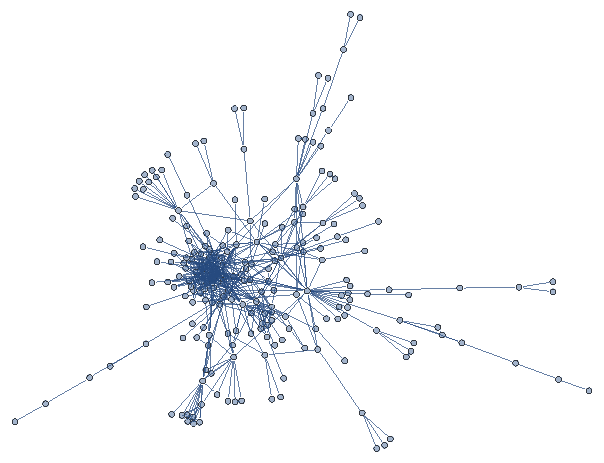
\includegraphics[width=0.45\textwidth]{../figures/graph_standard.pdf}
      };
    \end{scope}
    \begin{scope}[xshift=0.14\textwidth]
      \node [mybox] (box){
        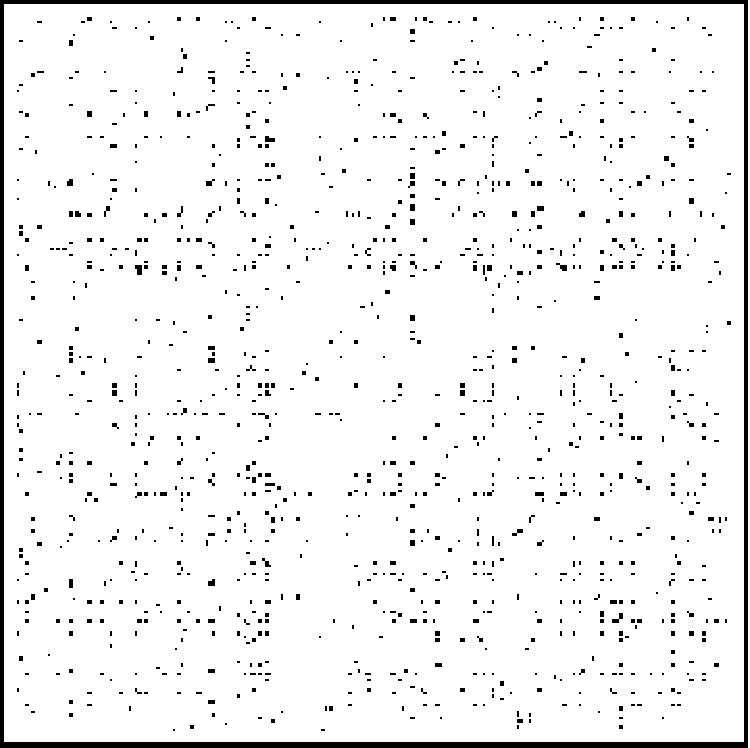
\includegraphics[width=0.36\textwidth]{../figures/unsorted_adjacency_matrix.pdf}
      };
    \end{scope}
  \end{scope}
%  \begin{scope}[yshift=-0.08\textwidth]
%    \begin{scope}[xshift=0cm]
%        \node[inner sep=0,text width=0.13\textwidth, text centered] (note1) at (0,0) {
%         \Large A protein interactome\ldots};
%     \end{scope}
%    \begin{scope}[xshift=0.14\textwidth]
%        \node[inner sep=0,text width=0.13\textwidth, text centered] (note1) at (0,0) {
%         \Large \ldots encoded as an array};
%     \end{scope}
%  \end{scope}
\end{tikzpicture}

  \end{block}
  \begin{block}{}
    In full generality, anything that can be stored in a relational database
  \end{block}
\end{frame}

\begin{frame}{How can we model such data?}
  \begin{block}{}
    \begin{itemize}
      \item Interested in generative modeling of such data for \eg
      \begin{itemize}
        \item Discovery of latent structure \eg groups of proteins with similar functions in protein-protein interactomes
        \item Prediction of missing data \eg movie recommendation, friend suggestions
      \end{itemize}
      \vspace{\baselineskip}
      \item Relational data typically encoded in arrays. How do reasonable assumptions about the data translate to the array representation
      \vspace{\baselineskip}
      \item We make a weak assumption and demonstrate the implied structure for arrays
      \begin{itemize}
        \item Implied structure allows for classification of many models
        \item Also inspires a simple Bayesian nonparametric model with good empirical performance
      \end{itemize}
    \end{itemize}
  \end{block}
\end{frame}

\begin{frame}{Exchangeability for relational data}
  \begin{block}{}
  \center
  \begin{tikzpicture}[scale=3]
  \begin{scope}[yshift=0cm]
    \tikzstyle{graph_node}=[circle,minimum size=0.045\textwidth,inner sep=0pt, fill=camlightblue]
    \def \radius {0.045\textwidth}
    \begin{scope}[xshift=0cm]
      \foreach \s in {1,...,10}
      {
        \node[draw, graph_node] (N\s) at ({360/10 * (\s - 1) + 90}:\radius) {\s};
      }   
      \path (N2) edge (N6);
      \path (N4) edge (N9);
      \path (N5) edge (N6);
      \path (N5) edge (N8);
      \path (N7) edge (N8);
      \path (N8) edge (N9);
      \path (N8) edge (N10);
      \path (N9) edge (N10);
    \end{scope}
    \begin{scope}[xshift=0.16\textwidth]
      \def \s {1}
      \node[draw, graph_node] (N\s) at ({360/10 * (\s - 1) + 90}:\radius) {2};
      \def \s {2}
      \node[draw, graph_node] (N\s) at ({360/10 * (\s - 1) + 90}:\radius) {7};
      \def \s {3}
      \node[draw, graph_node] (N\s) at ({360/10 * (\s - 1) + 90}:\radius) {6};
      \def \s {4}
      \node[draw, graph_node] (N\s) at ({360/10 * (\s - 1) + 90}:\radius) {5};
      \def \s {5}
      \node[draw, graph_node] (N\s) at ({360/10 * (\s - 1) + 90}:\radius) {3};
      \def \s {6}
      \node[draw, graph_node] (N\s) at ({360/10 * (\s - 1) + 90}:\radius) {1};
      \def \s {7}
      \node[draw, graph_node] (N\s) at ({360/10 * (\s - 1) + 90}:\radius) {10};
      \def \s {8}
      \node[draw, graph_node] (N\s) at ({360/10 * (\s - 1) + 90}:\radius) {8};
      \def \s {9}
      \node[draw, graph_node] (N\s) at ({360/10 * (\s - 1) + 90}:\radius) {4};
      \def \s {10}
      \node[draw, graph_node] (N\s) at ({360/10 * (\s - 1) + 90}:\radius) {9};
      \path (N2) edge (N6);
      \path (N4) edge (N9);
      \path (N5) edge (N6);
      \path (N5) edge (N8);
      \path (N7) edge (N8);
      \path (N8) edge (N9);
      \path (N8) edge (N10);
      \path (N9) edge (N10);
    \end{scope}
    \begin{scope}[xshift=0.08\textwidth]
      \node[inner sep=0,text width=0.13\textwidth, text centered,font=\Huge] (note1) at (0,0) {
         $\equiv$};
    \end{scope}
  \end{scope}
\end{tikzpicture}

  \end{block}
\end{frame}

\begin{frame}{Exchangeability for corresponding arrays}
  \begin{block}{}
  \center
  \begin{tikzpicture}[scale=3]
  \begin{scope}[yshift=0cm]
    \tikzstyle{graph_node}=[circle,minimum size=0.045\textwidth,inner sep=0pt, fill=camlightblue]
    \def \radius {0.045\textwidth}
    \begin{scope}[xshift=0cm]
      \foreach \s in {1,...,10}
      {
        \node[draw, graph_node] (N\s) at ({360/10 * (\s - 1) + 90}:\radius) {\s};
      }   
      \path (N2) edge (N6);
      \path (N4) edge (N9);
      \path (N5) edge (N6);
      \path (N5) edge (N8);
      \path (N7) edge (N8);
      \path (N8) edge (N9);
      \path (N8) edge (N10);
      \path (N9) edge (N10);
    \end{scope}
    \begin{scope}[xshift=0.16\textwidth]
      \def \s {1}
      \node[draw, graph_node] (N\s) at ({360/10 * (\s - 1) + 90}:\radius) {2};
      \def \s {2}
      \node[draw, graph_node] (N\s) at ({360/10 * (\s - 1) + 90}:\radius) {7};
      \def \s {3}
      \node[draw, graph_node] (N\s) at ({360/10 * (\s - 1) + 90}:\radius) {6};
      \def \s {4}
      \node[draw, graph_node] (N\s) at ({360/10 * (\s - 1) + 90}:\radius) {5};
      \def \s {5}
      \node[draw, graph_node] (N\s) at ({360/10 * (\s - 1) + 90}:\radius) {3};
      \def \s {6}
      \node[draw, graph_node] (N\s) at ({360/10 * (\s - 1) + 90}:\radius) {1};
      \def \s {7}
      \node[draw, graph_node] (N\s) at ({360/10 * (\s - 1) + 90}:\radius) {10};
      \def \s {8}
      \node[draw, graph_node] (N\s) at ({360/10 * (\s - 1) + 90}:\radius) {8};
      \def \s {9}
      \node[draw, graph_node] (N\s) at ({360/10 * (\s - 1) + 90}:\radius) {4};
      \def \s {10}
      \node[draw, graph_node] (N\s) at ({360/10 * (\s - 1) + 90}:\radius) {9};
      \path (N2) edge (N6);
      \path (N4) edge (N9);
      \path (N5) edge (N6);
      \path (N5) edge (N8);
      \path (N7) edge (N8);
      \path (N8) edge (N9);
      \path (N8) edge (N10);
      \path (N9) edge (N10);
    \end{scope}
    \begin{scope}[xshift=0.08\textwidth]
      \node[inner sep=0,text width=0.13\textwidth, text centered,font=\Huge] (note1) at (0,0) {
         $\equiv$};
    \end{scope}
  \end{scope}
  \begin{scope}[yshift=-0.12\textwidth]
    \begin{scope}[xshift=0cm]
      \node [mybox] (box){
        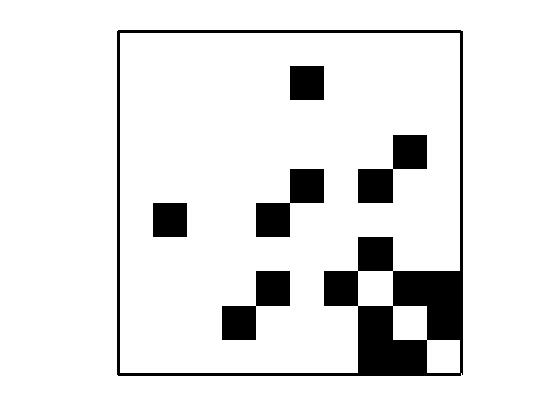
\includegraphics[width=0.45\textwidth]{../figures/adj.png}
      };
    \end{scope}
    \begin{scope}[xshift=0.16\textwidth]
      \node [mybox] (box){
        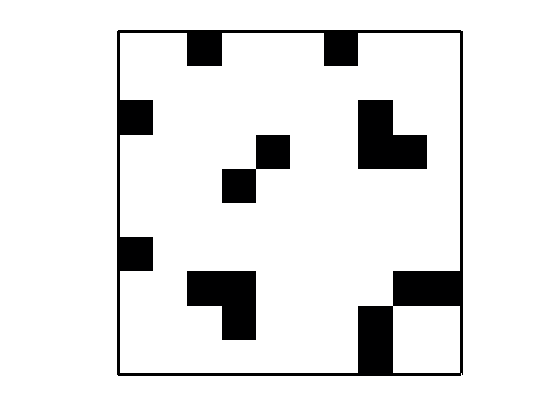
\includegraphics[width=0.45\textwidth]{../figures/adj_perm.png}
      };
    \end{scope}
    \begin{scope}[xshift=0.08\textwidth]
      \node[inner sep=0,text width=0.13\textwidth, text centered,font=\Huge] (note1) at (0,0) {
         $\equiv$};
    \end{scope}
  \end{scope}
\end{tikzpicture}

  \end{block}
\end{frame}

\begin{frame}{Exchangeability can be characterised}
\begin{block}{}
  \begin{definition*}
  An array $\darray=(\darray_{ij})_{i,j\in\Nats}$ is called an \emph{exchangeable array} if 
  \begin{equation*}
    \label{eq:jointly:ex}
    (\darray_{ij})\eqdist(\darray_{\pi(i)\pi(j)}) \qquad\text{ for every }\pi\in\SGinf\;.
  \end{equation*}
\end{definition*}
\end{block}

%\vspace{1\baselineskip}
\begin{block}{}
\begin{theorem*}[Aldous, Hoover]
  \label{theorem:ah}
  A random 2-array $(\darray_{ij})$ is exchangeable if and only if there is a random (measurable) function ${F:[0,1]^3\rightarrow\dataspace}$ such that 
  \begin{equation*}
    \label{eq:ah}
    (\darray_{ij})\eqdist (F(\AHvar_i,\AHvar_j,\AHvar_{ij})).
  \end{equation*}
for every collection  $(\AHvar_i)_{i\in\Nats}$ and $(\AHvar_{ij})_{i\le j\in\Nats}$ of \iid $\Uniform[0,1]$ random variables, where $\AHvar_{ji} = \AHvar_{ij}$ for $j < i \in \Nats$.
\end{theorem*}
\end{block}
\end{frame}

\begin{frame}{An arbitrarily good approximation}
  \begin{block}{This representation can be simplified}
Call an array $(\darray_{ij})$, \emph{simple} if it admits a representation
\[
(\darray_{ij}) \eqd (\Theta(\AHvar_{i},\AHvar_{j})) \nonumber
\]
Let $\Law(Y)$ be the law (distribution) of a random variable $Y$ and \\define $\chi_m X \defas (X_{ij}; \ i,j \le m )$.
\end{block}
\begin{block}{}
\begin{thm}[{Kallenberg}]
\label{theorem:simple}
Let $\darray$ be a $d$-dimensional exchangeable array in a Borel space $\dataspace$.  Then there exist some simple exchangeable arrays $X_1,X_2,\dotsc$ such that $\Law(\chi_m X_n) \textrm{ and } \Law(\chi_m X)$ are mutually absolutely continuous for all $m,n \in \Nats$ and the associated Radon--Nikodym derivatives converge uniformly to 1 as $n \to \infty$ for fixed $m$.
\end{thm}
  \end{block}
%  \begin{block}{\ldots allowing the following simplification}
%    We can produce arbitrarily good approximations to exchangeable arrays with functions of the form
%    \[
%      (\darray_{ij}) = (F(\AHvar_i,\AHvar_j)) \nonumber
%    \]
%  \end{block}
\end{frame}

\begin{frame}{This inspires a Bayesian nonparametric model}
\begin{block}{}
We decompose the function $F$ into two functions 
${\AHfunction:[0,1]^2\rightarrow\latentspace}$ 
and ${H:[0,1]\times\latentspace\rightarrow\dataspace}$ for a suitable space $\latentspace$\/, such that
\begin{equation*}
  \label{eq:decomposition}
  (\darray_{ij}) \eqd (F(\AHvar_i,\AHvar_j,\AHvar_{ij}))=(H(\AHvar_{ij},\AHfunction(\AHvar_i,\AHvar_j)))\;.
\end{equation*}
\end{block}
\begin{block}{}
Inspiring the following generative model
\begin{equation}
  \begin{split}
    \AHfunction\; &\sim\; \GP(0,\kernel) \\
    \AHvar_{1},\AHvar_{2},\ldots\; &\simiid\; \Uniform[0,1] \nonumber \\
    \darray_{ij}\,|W_{ij}\; &\sim\; \likelihood[\,.\,|W_{ij}]
  \end{split}
\end{equation}

\begin{center}
where $W_{ij}=\AHfunction(\AHvar_i,\AHvar_j)$.
\end{center}
\end{block}
\end{frame}

\begin{frame}{The model  in pictures}
 \begin{block}{}
   \begin{tikzpicture}[>=stealth,scale=2,transform canvas={xshift=2cm,yshift=1cm}]
  \begin{scope}[yshift=1cm]
    \node (text1) at (0.5,0) {$\Theta: [0,1]^2\newarrow[0,1] \text{ measurable and symmetric}$};
    \node (text2) at ($(text1)+(3,0)$) {$U_1,U_2,\ldots\simiid\Uniform[0,1]$};
    \node (text3) at ($(text1)+(1.3,-0.3)$) {$\mbox{Pr}\lbrace \text{edge } i,j\rbrace=\Theta(U_i,U_j)$};
  \end{scope}
  %% \begin{scope}[yshift=1cm]
  %%   \node (text1) at (1.7,0) {$\Theta: [0,1]^2\newarrow[0,1] \text{ measurable and symmetric}$};
  %%   \node (text2) at ($(text1)+(0,-0.3)$) {$U_1,U_2,\ldots\simiid\Uniform[0,1]$};
  %% \end{scope}
  \begin{scope}[yshift=0cm,xshift=0cm,scale=1.1]
  \begin{scope}
    \path[use as bounding box] (-0.5,0.5) rectangle (2.8,-1.5);
    \draw (0,0) --(0,-1) --(1,-1) --(1,0) --(0,0);
    %\draw (0,0)--(1,-1);
    \node[font=\scriptsize] at (0,0.1) {$0$};
    \node[font=\scriptsize] at (-0.1,0) {$0$};
    \node[font=\scriptsize] at (1,-1.1) {$1$};
    \node[font=\scriptsize] at (1.1,-1) {$1$};
    \draw [dashed] (0.2,0.1) -- (0.2,-1.1); \node at (0.2,0.2) {$U_i$};
    \draw [dashed] (-0.1,-0.2) -- (1.1,-0.2); \node at (-0.25,-0.2) {$U_i$};
    \draw [dashed] (0.65,0.1) -- (0.65,-1.1); \node at (0.65,0.2) {$U_j$};
    \draw [dashed] (-0.1,-0.65) -- (1.1,-0.65); \node at (-0.25,-0.65) {$U_j$};
    \node[circle,fill,scale=0.4,color=red] (red1) at (0.65,-0.2) {};
  \end{scope}
  \begin{scope}[yshift=-2cm]
    \draw (0,0)--(1,0);
    \draw (0,-0.05)--(0,0.05); \node at (0,-0.15) {$0$};
    \draw (1,-0.05)--(1,0.05); \node at (1,-0.15) {$1$};
    \node[circle,fill,scale=0.4,color=red] (red2) at (0.21,0) {};
    %\node[font=\scriptsize] at (0.48,-0.1) {$\mbox{Pr}\lbrace X_{ij}=1\rbrace=\Theta(U_i,U_j)$};
    \node[font=\scriptsize,color=blue!30!gray] (flipprob) at (0.21,-0.5) {$\mbox{Pr}\lbrace\text{edge } i,j\rbrace$};
    \draw[->,color=blue!30!gray] ($(flipprob.north)+(0,0)$)--($(red2.south)+(0,-0.03)$);
  \end{scope}
  \begin{scope}
  \draw[->] ($(red1.south east)+(0.01,-0.01)$) .. controls (1,-0.8) and (1,-1.2) .. ($(red2.north east)+(0.01,0.01)$);
  \draw (0.5,-1.5) node [fill=none] {$\Theta$};
  \end{scope}
   \end{scope}
  \begin{scope}[xshift=2.7cm,yshift=-0.55cm]
    \node [mybox] (box1){
  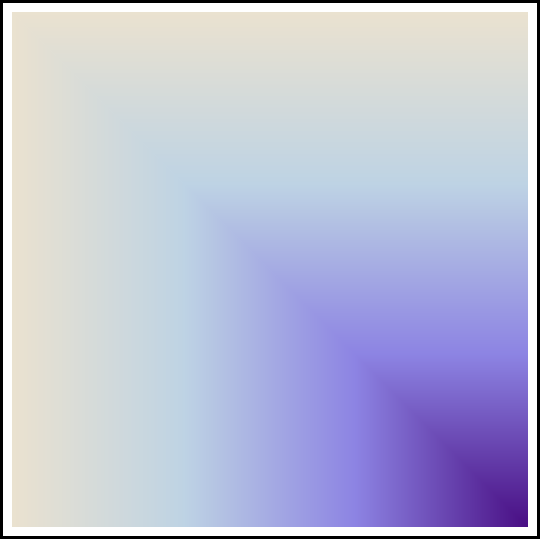
\includegraphics[width=2.24cm]{../figures/min_function.pdf} 
 %  \includegraphics[width=2.9cm]{include/uniform_attachment_graphon.pdf}
  };
    \node at ($(box1)+(0.7,0)$) {$\Theta$};
  \end{scope}  
  \begin{scope}[xshift=2.7cm,yshift=-2cm]
    \node [mybox] (box2){
      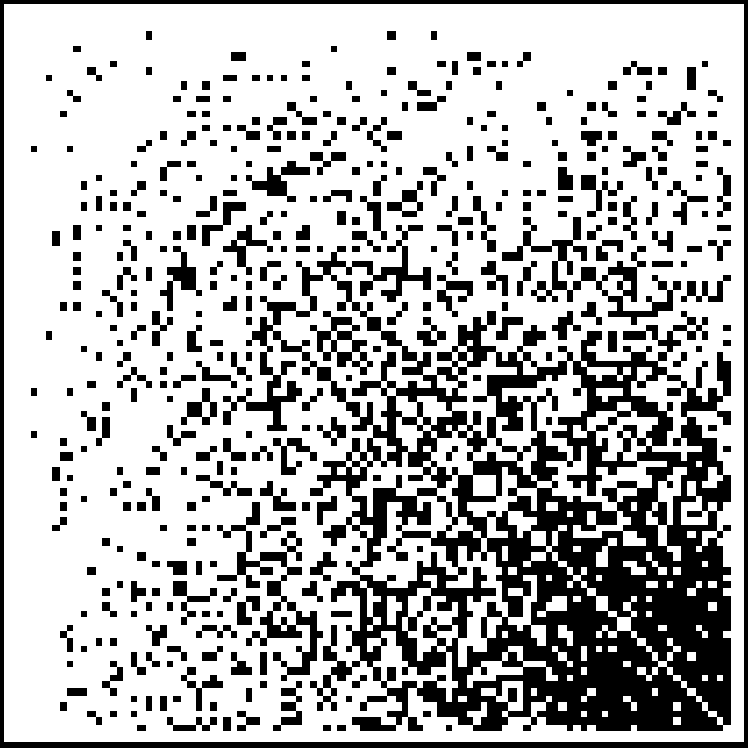
\includegraphics[width=2.24cm]{../figures/lovasz_sample100.pdf}
%    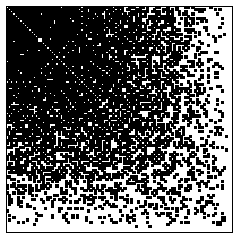
\includegraphics[width=2.8cm]{include/uniform_attachment_empirical.pdf}
  };
  \end{scope}
\end{tikzpicture}

 \end{block}
\end{frame}

\begin{frame}{Many models fit this pattern}
  \begin{block}{}
\begin{center}
  \begin{tabular}{lccl} 
%    \toprule
    \multicolumn{4}{c}{Graph data}\\
    \midrule
    %\addlinespace[2pt]
    %\textcolor{red}{Random function model} 
    Random function model & $\AHfunction$ & $\sim$ & $\GP\,(0, \kernel)$\\
    Latent class & $\larray_{ij}$ & $=$ & $\Lambda_{\AHvar_i\AHvar_j}\,\textrm{where} \,\AHvar_i \in \{1,\ldots,K\}$\\
    IRM & $\larray_{ij}$ & $=$ & $\Lambda_{\AHvar_i\AHvar_j}\,\textrm{where} \,\AHvar_i \in \{1,\ldots,\infty\}$\\
    Latent distance & $\larray_{ij}$ & $=$ & $-|\AHvar_i - \AHvar_j|$\\
    Eigenmodel &$\larray_{ij}$ & $=$ & $\AHvar_i'\Lambda \AHvar_j$\\
    LFRM & $\larray_{ij}$ & $=$ & $\AHvar_i'\Lambda \AHvar_j\,\textrm{where} \,\AHvar_i \in \{0,1\}^\infty$\\
    ILA & $\larray_{ij}$ & $=$ & $\sum_d \mathbb{I}_{U_{id}}\mathbb{I}_{U_{jd}}\Lambda^{(d)}_{U_{id}U_{jd}}\,\textrm{where} \,\AHvar_i \in \{0,\ldots,\infty\}^\infty$\\
    SMGB & $\AHfunction$ & $\dist$ & $\GP\,(0, \kernel_1 \otimes \kernel_2)$ \\
    %\midrule
    \addlinespace[4pt]
    \multicolumn{4}{c}{Real-valued array data}\\
    \midrule
    %\textcolor{red}{Random function model} 
    Random function model & $\AHfunction$ & $\sim$ & $\GP\,(0, \kernel)$\\
    Mondrian process based & $\AHfunction$ & = & piece-wise constant random function\\
    PMF & $\larray_{ij}$ & $=$ & $\AHvar_i'V_j$\\
    GPLVM & $\AHfunction$ & $\sim$ & $\GP\,(0, \kernel \otimes \delta)$\\
    %Linear relational GP~\cite{Yu2008} & $\AHfunction$ & $\sim$ & $\GP\,(0, \kernel_1 \otimes \kernel_2)\,\textrm{where} \,\kernel_i\,\textrm{is linear} $\\
%\bottomrule
\end{tabular}
\end{center}
  \end{block}
\end{frame}

\begin{frame}{A correspondence result}
  \begin{block}{}
\begin{prop}
\label{prop:matrixfactorisation}
A matrix factorization model defined as
\begin{equation*}
W_{ij} = \AHvar_i'\Lambda\AHvaralt_j \quad \quad \Lambda_{ij} \simiid \Normal (0, 1)
\end{equation*}
is equivalent to
\begin{equation*}
W_{ij} = \AHfunction\,(\AHvar_i, \AHvaralt_j) \quad \quad \AHfunction \sim \GP\,(0, L_\AHvar \otimes L_\AHvaralt)
\end{equation*}
\vspace{\baselineskip}

where $L_U(\AHvar_{i_1}, \AHvar_{i_2}) = \AHvar_{i_1}'\AHvar_{i_2}$ and similarly for $L_V$.
\end{prop}
  \end{block}
\end{frame}

\begin{frame}{A simpler overview of model space}
  \begin{block}{}
  \centering
  \begin{tabular}{l|ccc}%c} 
%    \toprule
    & $W_{ij}$ & $\kernel$ & $U_i, V_j \sim \, .$ \\% & $\dataspace$\\ 
    %\multicolumn{4}{c}{Graph data}\\
    \midrule
    %\addlinespace[2pt]
    %\textcolor{red}{Random function model} 
    Random function model & $\phi(U_i, V_j)'\Lambda$ & $\kernel_{U\times V}$ & Gaussian\\% & All\\
    SMGB, InfTucker & $\phi(\AHvar_i)'\Lambda\phi(\AHvaralt_j)$ & $\kernel_U \otimes \kernel_V$ & Laplace \\% & $\{0,1\},\, \Reals$\\
    GPLVM & $\phi(\AHvar_i)'\Lambda$ & $\kernel_\AHvar \otimes \delta_V$ & Gaussian \\% & All\\
    Eigenmodel & $\AHvar_i'\Lambda \AHvaralt_j$ & $L_U \otimes L_V$ & Gaussian \\% & All\\
    Linear relational GP & $\AHvar_i'\Lambda \AHvaralt_j$ & $L_U \otimes L_V$ & Gaussian \\% & $\{0,1\}$\\
    PCA, PMF & $\AHvar_i'\Lambda$ & $L_U \otimes \delta_V$ & Gaussian \\% & $\Reals$\\
    Latent distance & $-|\AHvar_i - \AHvar_j|$ & 0 & Gaussian \\% & $\{0,1\}$\\
    Mondrian process based & Decision tree & * & Uniform \\% & All\\
    \midrule
    Latent class & $\Lambda_{\AHvar_i\AHvar_j}$ & $\delta_{U\times U}$ & Multinomial \\% & $\{0,1\}$\\
    IRM &$\Lambda_{\AHvar_i\AHvaralt_j}$ & $\delta_{U\times V}$ & CRP \\% & $\{0,1\}$\\
    IHRM  &$\Lambda_{\AHvar_i\AHvaralt_j}$ & $\delta_{U\times V}$ & CRP \\% & $\Reals$\\
    BMF  & $\AHvar_i'\Lambda \AHvaralt_j$ & $L_U \otimes L_V$ & IBP \\% & $\Reals$\\
    LFRM & $\AHvar_i'\Lambda \AHvar_j$ & $L_U \otimes L_U$ & IBP \\% & $\{0,1\}$\\
    ILA & $\sum_d \mathbb{I}_{U_{id}}\mathbb{I}_{U_{jd}}\Lambda^{(d)}_{U_{id}U_{jd}}$ & * & CRP $+$ IBP \\% &$\{0,1\}$ \\
    %\midrule
    %\addlinespace[4pt]
    %\multicolumn{4}{c}{Real-valued matrix data}\\
    %\midrule
    %\textcolor{red}{Random function model} 
%\bottomrule
\end{tabular}
  \end{block}
\end{frame}

\begin{frame}{Posterior}
  \begin{block}{}
  \begin{center}
  \begin{tikzpicture}[scale=3]
  \begin{scope}[xshift=0cm]
    \node [mybox] (box){
      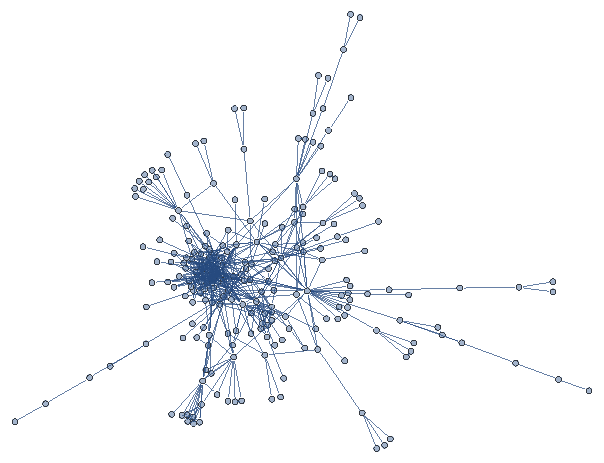
\includegraphics[width=0.3\textwidth]{../figures/graph_standard.pdf}
    };
    \node[inner sep=0,text width=0.3\textwidth, text centered] (note1) at (0,-0.06\textwidth) {
         A protein interactome};
  \end{scope}
  \begin{scope}[xshift=0.12\textwidth]
    \node [mybox] (box){
      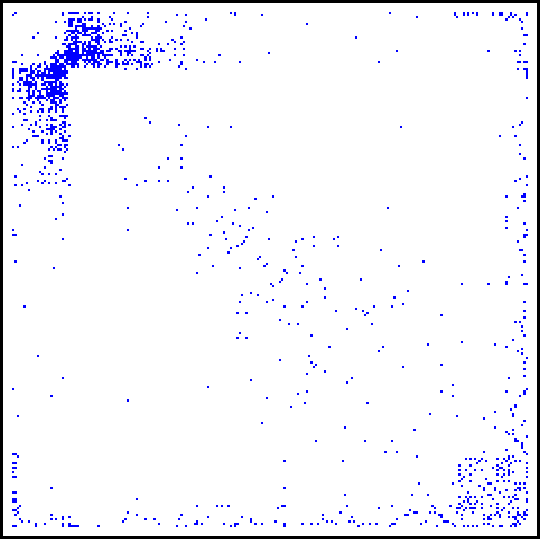
\includegraphics[width=0.24\textwidth]{../figures/interactome_adjacency_mathematica.pdf}
  };
    \node[inner sep=0,text width=0.3\textwidth, text centered] (note1) at (0,-0.06\textwidth) {
         Adjacency matrix sorted by MAP embedding};
  \end{scope}  
  \begin{scope}[xshift=0.24\textwidth]
    \node [mybox] (box){
      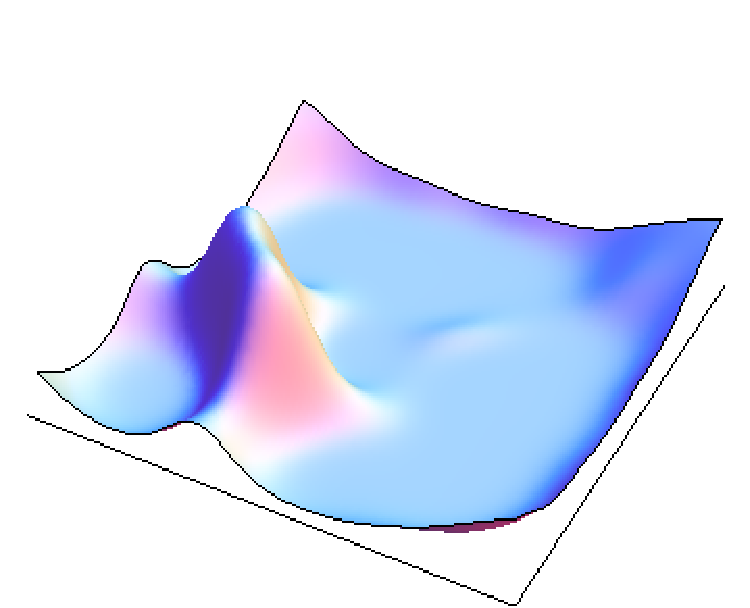
\includegraphics[width=0.3\textwidth]{../figures/graphon_listplot_bmp.pdf}
  };
    \node[inner sep=0,text width=0.3\textwidth, text centered] (note1) at (0,-0.06\textwidth) {
         MAP $\Theta$};
  \end{scope}
\end{tikzpicture}

\end{center}
  \end{block}
\end{frame}

\begin{frame}{Ongoing research / ideas}
  \begin{block}{}
    \begin{itemize}
      \item Modeling multiple arrays \eg joint modelling of social network and `like' data
      \begin{itemize}
        \item Corollaries of Aldous--Hoover suggest representations for such data
        \item Many unanswered questions about generating good models
      \end{itemize}
      \vspace{\baselineskip}
      \item Trying new priors on functions
      \begin{itemize}
        \item Many priors on functions for sequential data that could have utility for relational data
        \item \eg Analogous versions of $k$-means, mixture of Gaussians?
      \end{itemize}
      \vspace{\baselineskip}
      \item Trying new priors on latent variables
      \begin{itemize}
        \item CRP $+$ IBP prior in ILA could be more broadly applicable
      \end{itemize}
    \end{itemize}
  \end{block}
\end{frame}

\begin{frame}{Extensions: Array with `feature' data}
  \begin{block}{}
\begin{cor}
  \label{theorem:ahcov}
  Let $(\darray_{ij})_{i,j\in\Nats}$ and $(\CovData_i)_{i\in\Nats}$ be random variables in $\dataspace$ and $\dataspace'$ respectively.  Then the following are equivalent:
\begin{enumerate}  
\item[i.] $(\darray_{ij}, \CovData_i)\eqdist(\darray_{\pi(i)\pi(j)}, \CovData_{\pi(i)}) \,\text{ for every }\pi\in\SGinf$. 
\item[ii.] There are random (measurable) functions $F:[0,1]^3\rightarrow\dataspace$ and $G:[0,1]\rightarrow\dataspace'$ such that 
   \begin{equation}
    \label{eq:ah:cov}
    (\darray_{ij}, \CovData_i)\eqdist (F(\AHvar_i,\AHvar_j,\AHvar_{ij}), G(\AHvar_i)),
  \end{equation}
for every collection $(\AHvar_i)_{i\in\Nats}$ and $(\AHvar_{ij})_{i\le j\in\Nats}$ of \iid $\Uniform[0,1]$ random variables, where $\AHvar_{ji} = \AHvar_{ij}$ for $j < i \in \Nats$.
\end{enumerate}
\end{cor}
  \end{block}
\end{frame}

\begin{frame}{Extensions: Multiple arrays}
  \begin{block}{}
Consider rating data $(\darray_{ij})$ with users $i$ and movies $j$, with side information in the form of covariates for both users, $\CovData_i$, and movies, $\CovDataAlt_j$, and a social network $(S_{ik})$ over users $i,k$.
\end{block}
  \begin{block}{}
\begin{cor}
The following are equivalent
\begin{enumerate}
\item[i.] $
(\darray_{ij}, \CovData_i, \CovDataAlt_j, S_{ik}) \eqdist
(\darray_{\pi(i)\pi'(j)}, \CovData_{\pi(i)}, \CovDataAlt_{\pi'(j)}, S_{\pi(i)\pi(k)})$ 
for every $\pi,\pi' \in \SGinf$.
\item[ii.] There exist random functions $F,G,H,I$ such that
\[
(\darray_{ij}, \CovData_i, \CovDataAlt_j, S_{ik}) \eqdist (F(\AHvar_i,\AHvaralt_j,W_{ij}), G(\AHvar_i), H(\AHvaralt_j), I(\AHvar_i,\AHvar_k,\AHvar_{ik}))
\]
for every collection $(\AHvar_i)_{i\in\Nats}, (\AHvaralt_j)_{j\in\Nats}, (W_{ij})_{i, j\in\Nats}$ and $(\AHvar_{ik})_{i\le k\in\Nats}$ of \iid $\Uniform[0,1]$ random variables, where $\AHvar_{ki} = \AHvar_{ik}$ for $k < i \in \Nats$.
\end{enumerate}
\end{cor}
  \end{block}
\end{frame}

\begin{frame}{Multiple arrays: preliminary numerical results}
 \begin{block}{Data}
   \begin{itemize}
   \item A friend of friends network collected from last.FM ($S_{ik}$)
   \item A user $\times$ genre matrix: $X_{ij} = 1$ iff user $i$ has listened to genre $j$
   \end{itemize}
 \end{block}
 \begin{block}{Cold start task}
   \begin{itemize}
     \item Want to predict entire rows of $X_{ij}$ \ie recommendations for new users
     \item Consider jointly modelling the array
   \end{itemize}
 \end{block}
 \begin{block}{Preliminary numerical results promising}
   Insert a table and some comparisons
 \end{block}
\end{frame}

\begin{frame}{Multiple arrays: many open questions}
  \begin{block}{}
    \begin{itemize}
      \item Which designs of model will effectively model multiple arrays without having to `balance' or compromise?
      \begin{itemize}
        \item Flat clustering models seem especially inappropriate \eg IRM
        \item Multiple clustering models seem well suited
        \item How does this transfer to GP case - in particular, prior on length scales
      \end{itemize}
      \vspace{\baselineskip}
      \item Is generative modelling appropriate, or can we find more efficient models of conditional densities?
      \begin{itemize}
        \item What are appropriate representations for conditional densities?
      \end{itemize}
    \end{itemize}
  \end{block}
\end{frame}

\begin{frame}{Potential future research - 1-array -> 2-array}
  \begin{block}{}
    \eg Mixture of basis functions (motivate via Mondrian)
    
    Relational $k$-means
    
    Must be something interesting
  \end{block}
\end{frame}

\begin{frame}{Appendix: RFM numerical results}
  \begin{block}{}
    Table
  \end{block}
\end{frame}

\begin{frame}{Appendix: RFM posterior}
  \begin{block}{}
    Pictures
  \end{block}
\end{frame}

\begin{frame}{Appendix: RFM inference}
  \begin{block}{}
    Words and maths
  \end{block}
\end{frame}

\end{document}


